\documentclass[border=6pt]{standalone}
\usepackage{tikz}
\usepackage{amsmath}
\usepackage{mathpazo}
\usetikzlibrary{positioning, arrows.meta, fit, backgrounds}
\begin{document}
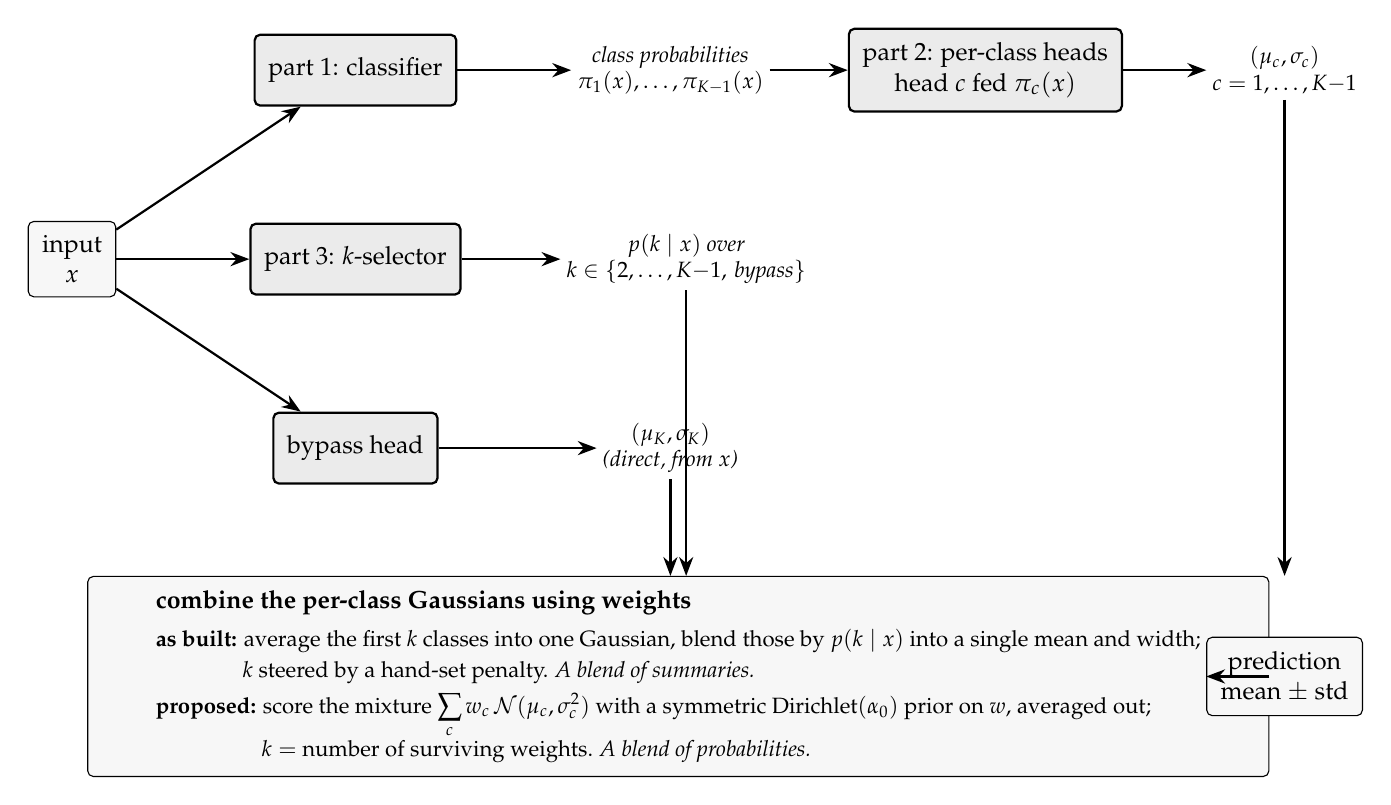
\begin{tikzpicture}[
  font=\small,
  >={Stealth[length=2.4mm]},
  box/.style   ={draw, rounded corners=2pt, align=center, inner sep=5pt, minimum height=9mm, fill=black!3},
  net/.style   ={draw, rounded corners=2pt, align=center, inner sep=5pt, minimum height=9mm, fill=black!8, thick},
  data/.style  ={align=center, inner sep=2pt, font=\footnotesize\itshape},
  arr/.style   ={->, thick},
]

% ---- input ----
\node[box] (x) at (0,0) {input\\$x$};

% ---- the three parts (column at x=3.4) ----
\node[net] (clf)  at (3.6, 2.4) {part 1: classifier};
\node[net] (ksel) at (3.6, 0.0) {part 3: $k$-selector};
\node[net] (byp)  at (3.6,-2.4) {bypass head};

\draw[arr] (x) -- (clf);
\draw[arr] (x) -- (ksel);
\draw[arr] (x) -- (byp);

% ---- pathway outputs ----
\node[data] (pi)   at (7.6, 2.4) {class probabilities\\$\pi_1(x),\dots,\pi_{K-1}(x)$};
\node[net]  (heads)at (11.6,2.4) {part 2: per-class heads\\head $c$ fed $\pi_c(x)$};
\node[data] (mus)  at (15.4,2.4) {$(\mu_c,\sigma_c)$\\$c=1,\dots,K{-}1$};
\draw[arr] (clf) -- (pi);
\draw[arr] (pi) -- (heads);
\draw[arr] (heads) -- (mus);

\node[data] (kp)   at (7.8, 0.0) {$p(k\mid x)$ over\\$k\in\{2,\dots,K{-}1,\,\text{bypass}\}$};
\draw[arr] (ksel) -- (kp);

\node[data] (bypout) at (7.6,-2.4) {$(\mu_K,\sigma_K)$\\(direct, from $x$)};
\draw[arr] (byp) -- (bypout);

% ---- combine box (wide, lower tier) ----
\node[box, minimum width=150mm, minimum height=22mm, align=left] (comb) at (7.7,-5.3)
  {\textbf{combine the per-class Gaussians using weights}\\[3pt]
   \footnotesize\textbf{as built:} average the first $k$ classes into one Gaussian, blend those by $p(k\mid x)$ into a single mean and width;\\
   \footnotesize\phantom{\textbf{as built:}} $k$ steered by a hand-set penalty. \emph{A blend of summaries.}\\[2pt]
   \footnotesize\textbf{proposed:} score the mixture $\displaystyle\sum_c w_c\,\mathcal{N}(\mu_c,\sigma_c^2)$ with a symmetric Dirichlet$(\alpha_0)$ prior on $w$, averaged out;\\
   \footnotesize\phantom{\textbf{proposed:}} $k=$ number of surviving weights. \emph{A blend of probabilities.}};

\draw[arr] (mus.south)   .. controls +(0,-1.2) and +(0,1.2) .. (comb.north -| mus.south);
\draw[arr] (kp.south)    -- (comb.north -| kp.south);
\draw[arr] (bypout.south).. controls +(0,-0.8) and +(0,1.2) .. (comb.north -| bypout.south);

% ---- output ----
\node[box] (out) at (15.4,-5.3) {prediction\\mean $\pm$ std};
\draw[arr] (comb.east) -- (out);

\end{tikzpicture}
\end{document}
